% SPDX-License-Identifier: MIT
% Copyright (c) 2017-2020 Forschungszentrum Juelich GmbH
% This code is licensed under MIT license (see the LICENSE file for details)
%
\documentclass{beamer}
\usetheme{Juelich}
% enable the \fzjset line to allow compat colors globally
% disabled by default since v18.10
\fzjset{compat mode=enabled}
\setlength{\abovecaptionskip}{0pt plus 0pt minus 0pt}

\bibliography{references.bib}
\usepackage{physics}

\title{GPU-Isle}
\author{Marcel, Stefan, Johann, Jan-Lukas}
\institute{JSC, JSC, Uni Bonn, ESS}
\date{\today}
\titlegraphic{\includegraphics%
    [width=\paperwidth]{placeholder}}
\begin{document}
\maketitle

\setbeamertemplate{caption}{\raggedright\insertcaption\par}
\begin{frame}{GPU-Isle Team}
\begin{columns}
\begin{column}{0.25\textwidth}
\begin{figure}

\includegraphics[width=4em,height=6em]{HackathonSlides/Pictures/Marcel_Rodekamp.jpg}
\caption{Marcel Rodekamp}
\end{figure}
\end{column}
\begin{column}{0.25\textwidth}
\begin{figure}
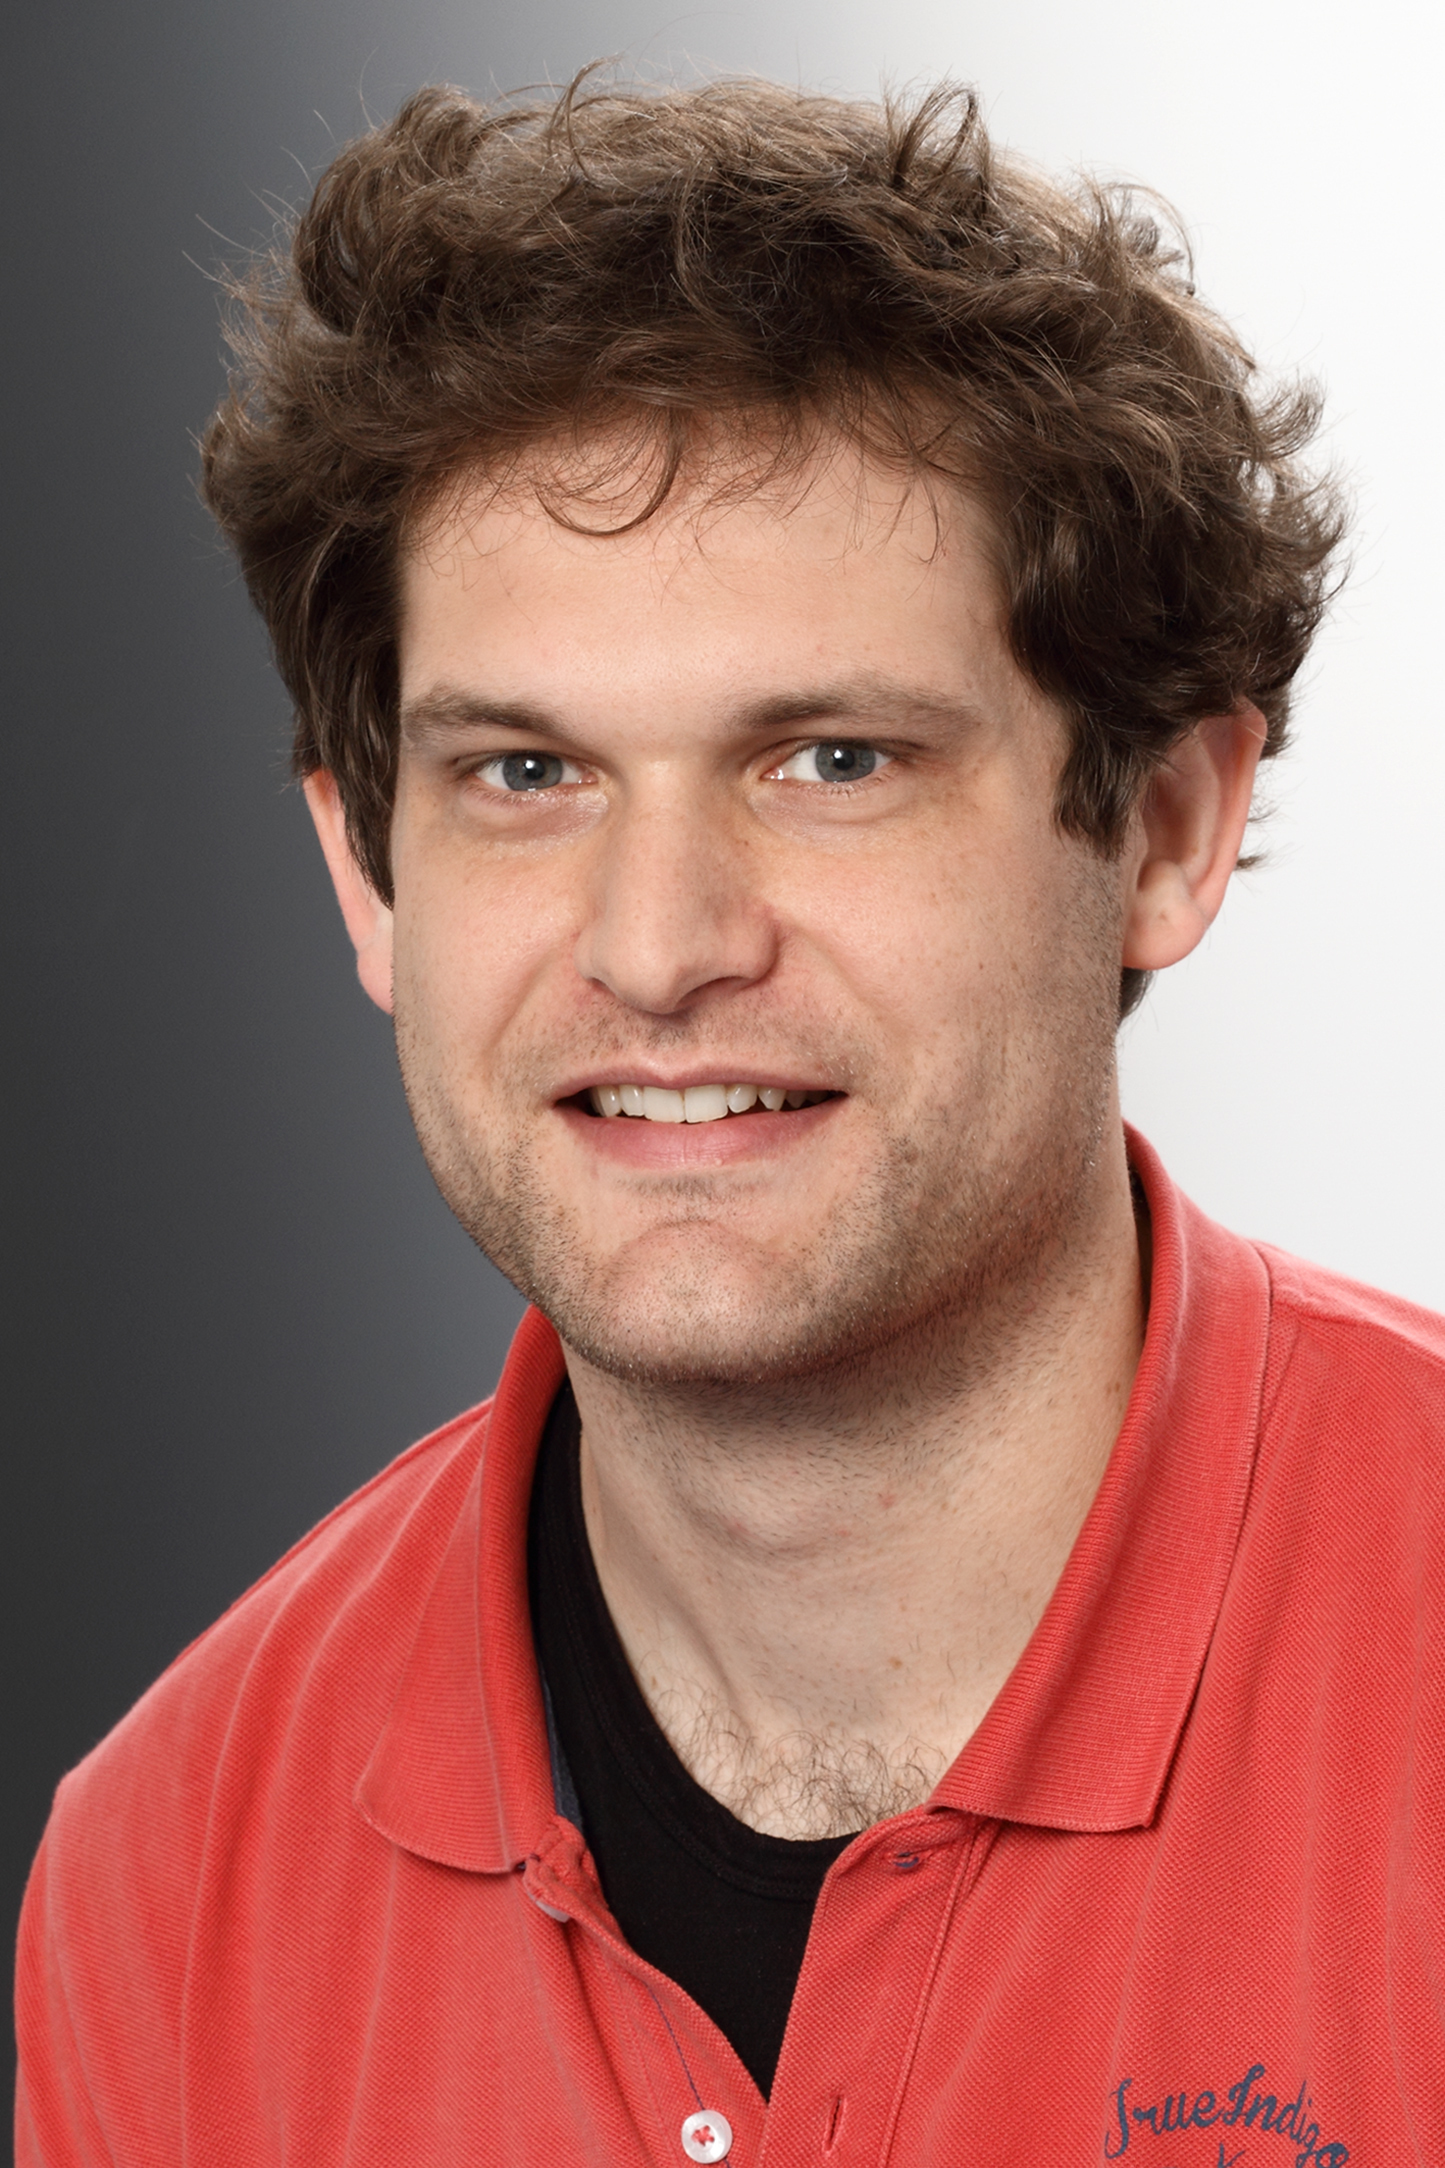
\includegraphics[width=5em,height=6em]{HackathonSlides/Pictures/krieg_009e.jpg}
\caption{Stefan Krieg}
\end{figure}
\end{column}
\begin{column}{0.25\textwidth}
\begin{figure}
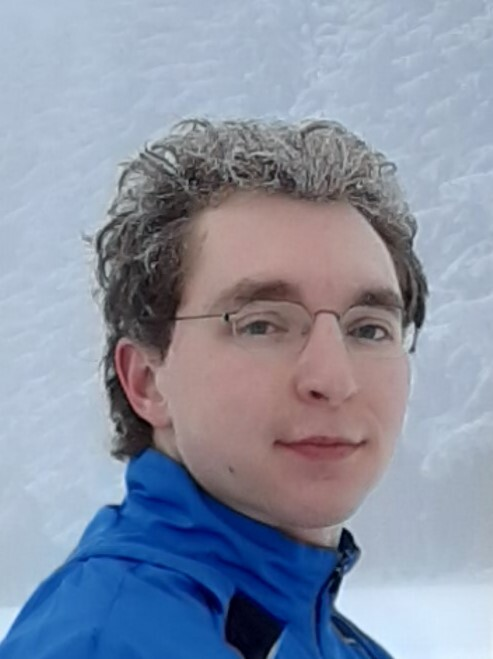
\includegraphics[width=5em,height=6em]{HackathonSlides/Pictures/johann_greiser_kopf.jpg}
\caption{Johann Ostmeyer}
\end{figure}
\end{column}
\begin{column}{0.25\textwidth}
\begin{figure}
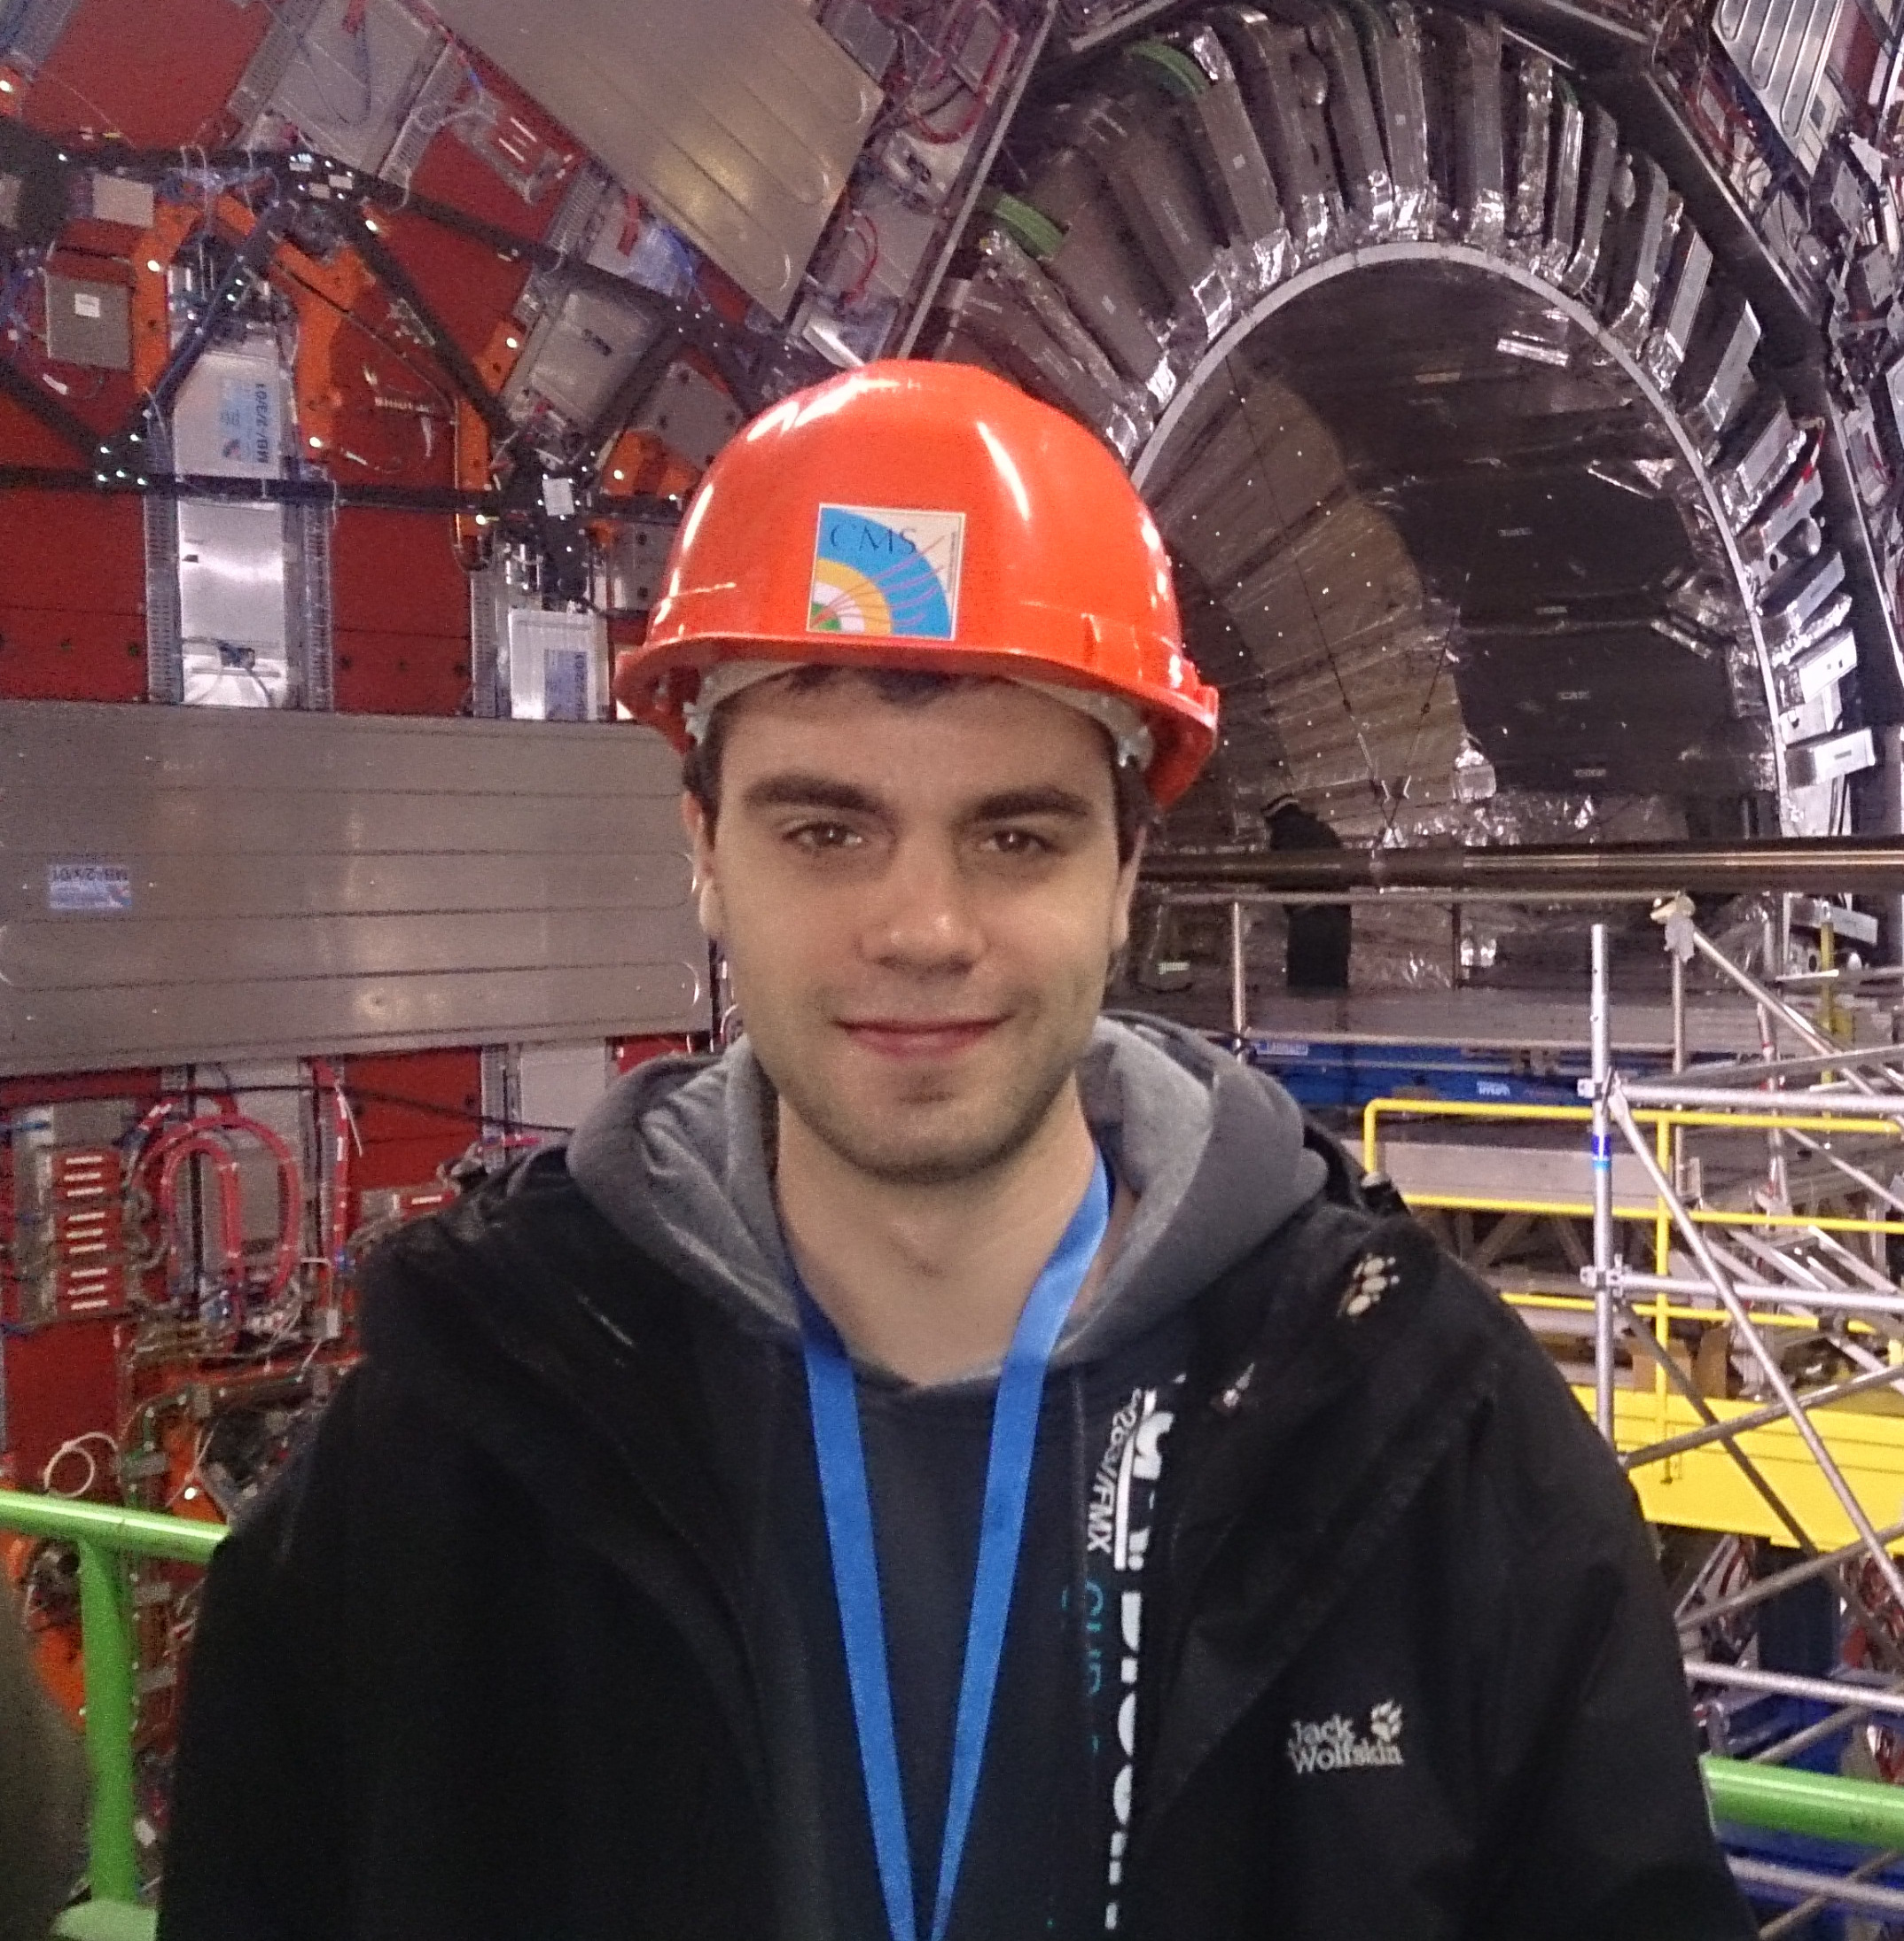
\includegraphics[width=6em,height=6em]{HackathonSlides/Pictures/DSC_0762.JPG}
\caption{Jan-Lukas Wynen}
\end{figure}
\end{column}
\end{columns}
\begin{columns}
\begin{column}{0.25\textwidth}
\begin{figure}
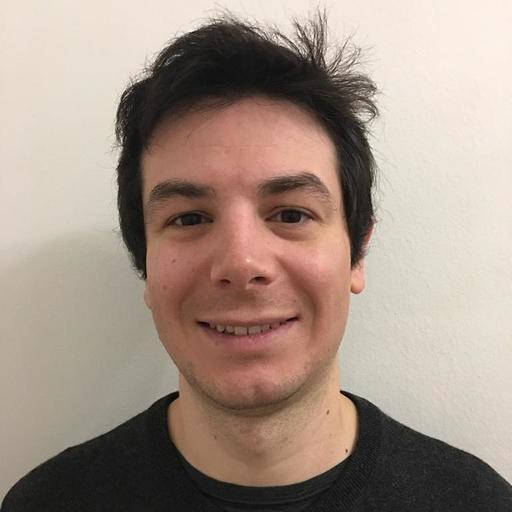
\includegraphics[width=6em,height=6em]{HackathonSlides/Pictures/Gonzalo.jpg}
\vspace*{-2em}
\caption{Gonzalo Brito}
\end{figure}
\end{column}
\begin{column}{0.25\textwidth}
\begin{figure}
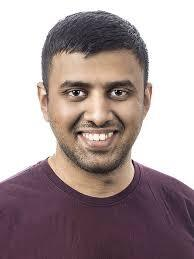
\includegraphics[width=5em,height=6em]{HackathonSlides/Pictures/jayesh.jpg}
\vspace*{-2em}
\caption{Jayesh Badwaik}
\end{figure}
\end{column}
\begin{column}{0.5\textwidth}

\end{column}
\end{columns}
\end{frame}
\setbeamertemplate{caption}[default]

\begin{frame}
    \frametitle{Simulating Carbon Nano Systems}
    \begin{columns}
    \begin{column}{0.5\textwidth}
        \begin{itemize}
            \item Lattices of carbon atoms
            \item Various geometries
            \item High technical interest
            \begin{itemize}
                \item Improved semiconductors
                \item Filtering techniques
            \end{itemize}
            \item Simulating behaviour: Quantum Field Theory
            \begin{itemize}
                \item[1.] System description with Energy functional (Hamiltonian)
                \only<1>{
                \item[2.] Generation of many states (Configurations)
                } \only<2> {
                \item[\textcolor{fzjred}{2.}] \textcolor{fzjred}{Generation of many states (Configurations)}
                }
                \item[3.] Evaluating physical quantities
            \end{itemize}
        \end{itemize}
    \end{column}
    \begin{column}{0.5\textwidth}
        \begin{figure}\centering
            \resizebox{0.5\textwidth}{!}{
            \begin{tikzpicture}
                \colorlet{vert}{fzjblack}
                \colorlet{edge}{fzjblue}
                \colorlet{back}{fzjgrey}
                \draw[draw=edge!42!back, line width=1.0, line cap=round] (0.3849, 0.2939) -- (-0.1405, 0.1148);
                \draw[draw=edge!42!back, line width=1.0, line cap=round] (-0.1405, 0.1148) -- (-0.2662, -0.4249);
                \draw[draw=edge!45!back, line width=1.0, line cap=round] (-0.1405, 0.1148) -- (-0.5704, 0.4226);
                \draw[draw=edge!46!back, line width=1.0, line cap=round] (0.7838, -0.0660) -- (0.3849, 0.2939);
                \draw[draw=edge!46!back, line width=1.0, line cap=round] (-0.2662, -0.4249) -- (0.1327, -0.7848);
                \draw[draw=edge!48!back, line width=1.0, line cap=round] (0.7838, -0.0660) -- (0.6578, -0.6056);
                \draw[draw=edge!48!back, line width=1.0, line cap=round] (0.6578, -0.6056) -- (0.1327, -0.7848);
                \draw[draw=edge!48!back, line width=1.0, line cap=round] (-0.2662, -0.4249) -- (-0.7744, -0.4501);
                \draw[draw=edge!48!back, line width=1.0, line cap=round] (0.4798, 0.7815) -- (0.3849, 0.2939);
                \draw[draw=edge!50!back, line width=1.0, line cap=round] (-0.5704, 0.4226) -- (-0.9625, 0.0735);
                \draw[draw=edge!50!back, line width=1.0, line cap=round] (-0.9625, 0.0735) -- (-0.7744, -0.4501);
                \draw[draw=edge!51!back, line width=1.0, line cap=round] (-0.4755, 0.9102) -- (-0.5704, 0.4226);
                \draw[draw=edge!53!back, line width=1.0, line cap=round] (0.4798, 0.7815) -- (0.0496, 1.0894);
                \draw[draw=edge!53!back, line width=1.0, line cap=round] (0.0496, 1.0894) -- (-0.4755, 0.9102);
                \draw[draw=edge!55!back, line width=1.0, line cap=round] (0.7838, -0.0660) -- (1.1254, 0.1987);
                \draw[draw=edge!56!back, line width=1.0, line cap=round] (0.1327, -0.7848) -- (0.0236, -1.1704);
                \draw[draw=edge!56!back, line width=1.0, line cap=round] (1.1254, 0.1987) -- (0.9373, 0.7228);
                \draw[draw=edge!56!back, line width=1.0, line cap=round] (0.9373, 0.7228) -- (0.4798, 0.7815);
                \draw[draw=edge!58!back, line width=1.0, line cap=round] (-0.7744, -0.4501) -- (-0.8835, -0.8358);
                \draw[draw=edge!59!back, line width=1.0, line cap=round] (0.6578, -0.6056) -- (0.8731, -0.8800);
                \draw[draw=edge!61!back, line width=1.0, line cap=round] (-0.9625, 0.0735) -- (-1.2594, 0.2118);
                \draw[draw=edge!62!back, line width=1.0, line cap=round] (0.0236, -1.1704) -- (-0.4846, -1.1957);
                \draw[draw=edge!62!back, line width=1.0, line cap=round] (-0.8835, -0.8358) -- (-0.4846, -1.1957);
                \draw[draw=edge!63!back, line width=1.0, line cap=round] (-0.4755, 0.9102) -- (-0.7726, 1.0485);
                \draw[draw=edge!64!back, line width=1.0, line cap=round] (0.8731, -0.8800) -- (0.4816, -1.2293);
                \draw[draw=edge!64!back, line width=1.0, line cap=round] (0.0236, -1.1704) -- (0.4816, -1.2293);
                \draw[draw=edge!66!back, line width=1.0, line cap=round] (0.0768, 1.3386) -- (0.0496, 1.0894);
                \draw[draw=edge!66!back, line width=1.0, line cap=round] (1.3407, -0.0756) -- (1.1254, 0.1987);
                \draw[draw=edge!67!back, line width=1.0, line cap=round] (-0.7726, 1.0485) -- (-1.1645, 0.6993);
                \draw[draw=edge!67!back, line width=1.0, line cap=round] (-1.1645, 0.6993) -- (-1.2594, 0.2118);
                \draw[draw=edge!68!back, line width=1.0, line cap=round] (0.8731, -0.8800) -- (1.2150, -0.6149);
                \draw[draw=edge!68!back, line width=1.0, line cap=round] (1.2150, -0.6149) -- (1.3407, -0.0756);
                \draw[draw=edge!69!back, line width=1.0, line cap=round] (0.9373, 0.7228) -- (0.9650, 0.9718);
                \draw[draw=edge!69!back, line width=1.0, line cap=round] (-0.8835, -0.8358) -- (-1.1806, -0.6974);
                \draw[draw=edge!71!back, line width=1.0, line cap=round] (-1.2594, 0.2118) -- (-1.3684, -0.1735);
                \draw[draw=edge!71!back, line width=1.0, line cap=round] (-1.3684, -0.1735) -- (-1.1806, -0.6974);
                \draw[draw=edge!71!back, line width=1.0, line cap=round] (0.0768, 1.3386) -- (-0.4309, 1.3132);
                \draw[draw=edge!71!back, line width=1.0, line cap=round] (-0.4309, 1.3132) -- (-0.7726, 1.0485);
                \draw[draw=edge!73!back, line width=1.0, line cap=round] (0.9650, 0.9718) -- (0.5348, 1.2798);
                \draw[draw=edge!73!back, line width=1.0, line cap=round] (0.5348, 1.2798) -- (0.0768, 1.3386);
                \draw[draw=edge!76!back, line width=1.0, line cap=round] (-0.4846, -1.1957) -- (-0.5348, -1.2798);
                \draw[draw=edge!78!back, line width=1.0, line cap=round] (0.4816, -1.2293) -- (0.4309, -1.3132);
                \draw[draw=edge!78!back, line width=1.0, line cap=round] (1.3407, -0.0756) -- (1.3684, 0.1735);
                \draw[draw=edge!80!back, line width=1.0, line cap=round] (1.3684, 0.1735) -- (1.1806, 0.6974);
                \draw[draw=edge!80!back, line width=1.0, line cap=round] (1.1806, 0.6974) -- (0.9650, 0.9718);
                \draw[draw=edge!80!back, line width=1.0, line cap=round] (-0.5348, -1.2798) -- (-0.9650, -0.9718);
                \draw[draw=edge!80!back, line width=1.0, line cap=round] (-1.1806, -0.6974) -- (-0.9650, -0.9718);
                \draw[draw=edge!81!back, line width=1.0, line cap=round] (-1.1645, 0.6993) -- (-1.2150, 0.6149);
                \draw[draw=edge!82!back, line width=1.0, line cap=round] (1.2150, -0.6149) -- (1.1645, -0.6993);
                \draw[draw=edge!83!back, line width=1.0, line cap=round] (-1.3684, -0.1735) -- (-1.3407, 0.0756);
                \draw[draw=edge!83!back, line width=1.0, line cap=round] (-1.2150, 0.6149) -- (-1.3407, 0.0756);
                \draw[draw=edge!83!back, line width=1.0, line cap=round] (0.4309, -1.3132) -- (-0.0768, -1.3386);
                \draw[draw=edge!83!back, line width=1.0, line cap=round] (-0.5348, -1.2798) -- (-0.0768, -1.3386);
                \draw[draw=edge!85!back, line width=1.0, line cap=round] (-0.4816, 1.2293) -- (-0.4309, 1.3132);
                \draw[draw=edge!86!back, line width=1.0, line cap=round] (0.4309, -1.3132) -- (0.7726, -1.0485);
                \draw[draw=edge!86!back, line width=1.0, line cap=round] (0.7726, -1.0485) -- (1.1645, -0.6993);
                \draw[draw=edge!87!back, line width=1.0, line cap=round] (0.5348, 1.2798) -- (0.4843, 1.1958);
                \draw[draw=edge!88!back, line width=1.0, line cap=round] (1.1645, -0.6993) -- (1.2594, -0.2118);
                \draw[draw=edge!88!back, line width=1.0, line cap=round] (1.2594, -0.2118) -- (1.3684, 0.1735);
                \draw[draw=edge!90!back, line width=1.0, line cap=round] (-0.4816, 1.2293) -- (-0.8731, 0.8800);
                \draw[draw=edge!90!back, line width=1.0, line cap=round] (-0.8731, 0.8800) -- (-1.2150, 0.6149);
                \draw[draw=edge!91!back, line width=1.0, line cap=round] (1.1806, 0.6974) -- (0.8835, 0.8358);
                \draw[draw=edge!91!back, line width=1.0, line cap=round] (0.8835, 0.8358) -- (0.4843, 1.1958);
                \draw[draw=edge!93!back, line width=1.0, line cap=round] (-0.9650, -0.9718) -- (-0.9373, -0.7228);
                \draw[draw=edge!93!back, line width=1.0, line cap=round] (0.4843, 1.1958) -- (-0.0236, 1.1704);
                \draw[draw=edge!93!back, line width=1.0, line cap=round] (-0.0236, 1.1704) -- (-0.4816, 1.2293);
                \draw[draw=edge!94!back, line width=1.0, line cap=round] (-0.9373, -0.7228) -- (-1.1251, -0.1989);
                \draw[draw=edge!94!back, line width=1.0, line cap=round] (-1.3407, 0.0756) -- (-1.1251, -0.1989);
                \draw[draw=edge!96!back, line width=1.0, line cap=round] (-0.0768, -1.3386) -- (-0.0496, -1.0894);
                \draw[draw=edge!98!back, line width=1.0, line cap=round] (0.7726, -1.0485) -- (0.4755, -0.9102);
                \draw[draw=edge!98!back, line width=1.0, line cap=round] (-0.0496, -1.0894) -- (0.4755, -0.9102);
                \draw[draw=edge!99!back, line width=1.0, line cap=round] (1.2594, -0.2118) -- (0.9625, -0.0735);
                \draw[draw=edge!101!back, line width=1.0, line cap=round] (-0.0496, -1.0894) -- (-0.4798, -0.7815);
                \draw[draw=edge!101!back, line width=1.0, line cap=round] (-0.9373, -0.7228) -- (-0.4798, -0.7815);
                \draw[draw=edge!101!back, line width=1.0, line cap=round] (0.9625, -0.0735) -- (0.7744, 0.4501);
                \draw[draw=edge!101!back, line width=1.0, line cap=round] (0.7744, 0.4501) -- (0.8835, 0.8358);
                \draw[draw=edge!101!back, line width=1.0, line cap=round] (-0.6575, 0.6055) -- (-0.8731, 0.8800);
                \draw[draw=edge!103!back, line width=1.0, line cap=round] (-0.0236, 1.1704) -- (-0.1327, 0.7848);
                \draw[draw=edge!103!back, line width=1.0, line cap=round] (-0.1327, 0.7848) -- (-0.6575, 0.6055);
                \draw[draw=edge!103!back, line width=1.0, line cap=round] (-0.6575, 0.6055) -- (-0.7838, 0.0660);
                \draw[draw=edge!103!back, line width=1.0, line cap=round] (-1.1251, -0.1989) -- (-0.7838, 0.0660);
                \draw[draw=edge!104!back, line width=1.0, line cap=round] (0.4755, -0.9102) -- (0.5704, -0.4226);
                \draw[draw=edge!104!back, line width=1.0, line cap=round] (0.5704, -0.4226) -- (0.9625, -0.0735);
                \draw[draw=edge!107!back, line width=1.0, line cap=round] (0.7744, 0.4501) -- (0.2664, 0.4248);
                \draw[draw=edge!107!back, line width=1.0, line cap=round] (0.2664, 0.4248) -- (-0.1327, 0.7848);
                \draw[draw=edge!107!back, line width=1.0, line cap=round] (-0.4798, -0.7815) -- (-0.3849, -0.2939);
                \draw[draw=edge!107!back, line width=1.0, line cap=round] (-0.3849, -0.2939) -- (-0.7838, 0.0660);
                \draw[draw=edge!109!back, line width=1.0, line cap=round] (0.5704, -0.4226) -- (0.1405, -0.1148);
                \draw[draw=edge!109!back, line width=1.0, line cap=round] (-0.3849, -0.2939) -- (0.1405, -0.1148);
                \draw[draw=edge!109!back, line width=1.0, line cap=round] (0.1405, -0.1148) -- (0.2664, 0.4248);
            \end{tikzpicture}
            }
            \caption{Graphical representation of a $C_{60}$ (Buckminsterfullerene) system. Each node represents a carbon atom and each edge the bond between two atoms.}
        \end{figure}
    \end{column}
    \end{columns}
\end{frame}

\begin{frame}\frametitle{The Hybrid Monte Carlo Algorithm}
\begin{columns}
\begin{column}[t]{0.6\textwidth}
    \begin{itemize}
        \item Building Markov Chain
        \item Iteratively updating previous configuration
        \item Update by Molecular Dynamics
        \begin{itemize}
            \item Integrate Hamilton equations
            \begin{itemize}
                \item \textbf{Leapfrog}
            \end{itemize}
            \item Requires: Matrix inversion
            \item Requires: Matrix, vector operations
        \end{itemize}
        \item Dimension $N_\tau\times \order{N_\sigma} $
        \begin{itemize}
            \item $C_{60}: \, N_\tau\times\order{60} $
        \end{itemize}
    \end{itemize}
\end{column}
\begin{column}[t]{0.4\textwidth}
    \begin{figure}
        \resizebox{\textwidth}{!}{
        \begin{tikzpicture}[node distance = 6em]
            \node[draw=fzjblue, rectangle, rounded corners, thick, align = center, text width = 8em] (input) {Input: \\ Configuration $\Phi_i$};
            \node[draw=fzjblue, rectangle, rounded corners, thick, align = center, text width = 8em, below of = input] (MD) {Molecular Dynamics: \\ $\Phi_i \mapsto \Phi_{i+1}^*$};
            \node[draw=fzjblue, rectangle, rounded corners, thick, align = center, text width = 8em, below of = MD, xshift = -6em] (MHA) {Accept:\\ $\Phi_{i+1} = \Phi_{i+1}^*$};
            \node[draw=fzjblue, rectangle, rounded corners, thick, align = center, text width = 8em, below of = MD, xshift =  6em] (MHR) {Reject:\\ $\Phi_{i+1} = \Phi_{i}$};

            \draw[->,>=stealth,thick] (input) -- (MD);
            \draw[->,>=stealth,thick] (MD.south) -- (MHA);
            \draw[->,>=stealth,thick] (MD.south) -- (MHR);
            \draw[->,>=stealth,thick] (MHA) |- (input);
            \draw[->,>=stealth,thick] (MHR) |- (input);
    \end{tikzpicture}
    }
    \end{figure}
\end{column}
\end{columns}
\end{frame}

\begin{frame}\frametitle{Isle}

    \begin{columns}
    \begin{column}[t]{0.5\textwidth}
        \centering
        \textbf{Current State}
        \begin{itemize}
            \item C++: Heavy math
            \item Python: Interface
            \item Build upon
            \begin{itemize}
                \item Blaze
                \item Lapack
            \end{itemize}
        \end{itemize}
    \end{column}
    \begin{column}[t]{0.5\textwidth}
        \centering
        \textbf{Goal}
        \begin{itemize}
            \item Port of Molecular Dynamics
            \begin{itemize}
                \item Leapfrog
                \item Matrix inverter
                \item Matrix, vector operations
            \end{itemize}
            \item Hybridization of Infrastructure (CPU,GPU)
            \item C++ with CUDA
            \item Blaze: CUDA Managed Pointer
            \item Utilize CUDA Math Libraries
        \end{itemize}
    \end{column}
    \end{columns}
\end{frame}

%\begin{frame}\frametitle{Isle - A Carbon Nano System Simulator}
%\begin{itemize}
%    \item Simulating Carbon Nano Systems
%    \item Basic Algorithm: Hybrid Monte Carlo
%\end{itemize}
%    \begin{figure}
%        \resizebox{0.6\textwidth}{!}{
%    \begin{tikzpicture}[node distance = 6em]
%        \node[draw=fzjblue, rectangle, rounded corners, thick, align = center, text width = 8em] (input) {Input: \\ Snapshot $\Phi_i$};
%        \uncover<2->{
%        \node[draw=fzjblue, rectangle, rounded corners, thick, align = center, text width = 8em, below of = input] (MD) {Molecular Dynamics (PDV): \\ $\Phi_i \mapsto \Phi_{i+1}^*$};
%        }
%        \uncover<3->{
%        \node[draw=fzjblue, rectangle, rounded corners, thick, align = center, text width = 8em, below of = MD, xshift = -6em] (MHA) {Accept:\\ $\Phi_{i+1} = \Phi_{i+1}^*$};
%        \node[draw=fzjblue, rectangle, rounded corners, thick, align = center, text width = 8em, below of = MD, xshift =  6em] (MHR) {Reject:\\ $\Phi_{i+1} = \Phi_{i}$};
%        }
%
%        \uncover<2->{\draw[->,>=stealth,thick] (input) -- (MD);}
%        \uncover<3->{\draw[->,>=stealth,thick] (MD.south) -- (MHA);}
%        \uncover<3->{\draw[->,>=stealth,thick] (MD.south) -- (MHR);}
%        \uncover<4->{\draw[->,>=stealth,thick] (MHA) |- (input);
%                     \draw[->,>=stealth,thick] (MHR) |- (input);}
%    \end{tikzpicture}
%    }
%    \end{figure}
%\end{frame}
%
%\begin{frame}
%    \frametitle{Isle Factsheet}
%    \begin{columns}
%    \begin{column}[t]{0.5\textwidth}
%        \centering
%        \textbf{Current State}
%        \begin{itemize}
%            \item C++ interfaced to Python
%            \item Build upon Blaze, BLAS
%        \end{itemize}
%    \end{column}
%    \begin{column}[t]{0.5\textwidth}
%        \centering
%        \textbf{Goal}
%        \begin{itemize}
%            \item Port of Molecular Dynamics
%            \item Hybridization of Infrastructure (CPU,GPU)
%            \item C++ with CUDA
%        \end{itemize}
%    \end{column}
%    \end{columns}
%    \par\bigskip
%\begin{itemize}
%    \item Benchmark System: Buckminsterfullerene $C_{60}$
%    \begin{itemize}
%        \item Informally called buckyballs
%    \end{itemize}
%\end{itemize}
%\begin{figure}
%\resizebox{0.2\textwidth}{!}{
%\begin{tikzpicture}
%    \colorlet{vert}{fzjblack}
%    \colorlet{edge}{fzjblue}
%    \colorlet{back}{fzjgrey}
%    \draw[draw=edge!42!back, line width=1.0, line cap=round] (0.3849, 0.2939) -- (-0.1405, 0.1148);
%    \draw[draw=edge!42!back, line width=1.0, line cap=round] (-0.1405, 0.1148) -- (-0.2662, -0.4249);
%    \draw[draw=edge!45!back, line width=1.0, line cap=round] (-0.1405, 0.1148) -- (-0.5704, 0.4226);
%    \draw[draw=edge!46!back, line width=1.0, line cap=round] (0.7838, -0.0660) -- (0.3849, 0.2939);
%    \draw[draw=edge!46!back, line width=1.0, line cap=round] (-0.2662, -0.4249) -- (0.1327, -0.7848);
%    \draw[draw=edge!48!back, line width=1.0, line cap=round] (0.7838, -0.0660) -- (0.6578, -0.6056);
%    \draw[draw=edge!48!back, line width=1.0, line cap=round] (0.6578, -0.6056) -- (0.1327, -0.7848);
%    \draw[draw=edge!48!back, line width=1.0, line cap=round] (-0.2662, -0.4249) -- (-0.7744, -0.4501);
%    \draw[draw=edge!48!back, line width=1.0, line cap=round] (0.4798, 0.7815) -- (0.3849, 0.2939);
%    \draw[draw=edge!50!back, line width=1.0, line cap=round] (-0.5704, 0.4226) -- (-0.9625, 0.0735);
%    \draw[draw=edge!50!back, line width=1.0, line cap=round] (-0.9625, 0.0735) -- (-0.7744, -0.4501);
%    \draw[draw=edge!51!back, line width=1.0, line cap=round] (-0.4755, 0.9102) -- (-0.5704, 0.4226);
%    \draw[draw=edge!53!back, line width=1.0, line cap=round] (0.4798, 0.7815) -- (0.0496, 1.0894);
%    \draw[draw=edge!53!back, line width=1.0, line cap=round] (0.0496, 1.0894) -- (-0.4755, 0.9102);
%    \draw[draw=edge!55!back, line width=1.0, line cap=round] (0.7838, -0.0660) -- (1.1254, 0.1987);
%    \draw[draw=edge!56!back, line width=1.0, line cap=round] (0.1327, -0.7848) -- (0.0236, -1.1704);
%    \draw[draw=edge!56!back, line width=1.0, line cap=round] (1.1254, 0.1987) -- (0.9373, 0.7228);
%    \draw[draw=edge!56!back, line width=1.0, line cap=round] (0.9373, 0.7228) -- (0.4798, 0.7815);
%    \draw[draw=edge!58!back, line width=1.0, line cap=round] (-0.7744, -0.4501) -- (-0.8835, -0.8358);
%    \draw[draw=edge!59!back, line width=1.0, line cap=round] (0.6578, -0.6056) -- (0.8731, -0.8800);
%    \draw[draw=edge!61!back, line width=1.0, line cap=round] (-0.9625, 0.0735) -- (-1.2594, 0.2118);
%    \draw[draw=edge!62!back, line width=1.0, line cap=round] (0.0236, -1.1704) -- (-0.4846, -1.1957);
%    \draw[draw=edge!62!back, line width=1.0, line cap=round] (-0.8835, -0.8358) -- (-0.4846, -1.1957);
%    \draw[draw=edge!63!back, line width=1.0, line cap=round] (-0.4755, 0.9102) -- (-0.7726, 1.0485);
%    \draw[draw=edge!64!back, line width=1.0, line cap=round] (0.8731, -0.8800) -- (0.4816, -1.2293);
%    \draw[draw=edge!64!back, line width=1.0, line cap=round] (0.0236, -1.1704) -- (0.4816, -1.2293);
%    \draw[draw=edge!66!back, line width=1.0, line cap=round] (0.0768, 1.3386) -- (0.0496, 1.0894);
%    \draw[draw=edge!66!back, line width=1.0, line cap=round] (1.3407, -0.0756) -- (1.1254, 0.1987);
%    \draw[draw=edge!67!back, line width=1.0, line cap=round] (-0.7726, 1.0485) -- (-1.1645, 0.6993);
%    \draw[draw=edge!67!back, line width=1.0, line cap=round] (-1.1645, 0.6993) -- (-1.2594, 0.2118);
%    \draw[draw=edge!68!back, line width=1.0, line cap=round] (0.8731, -0.8800) -- (1.2150, -0.6149);
%    \draw[draw=edge!68!back, line width=1.0, line cap=round] (1.2150, -0.6149) -- (1.3407, -0.0756);
%    \draw[draw=edge!69!back, line width=1.0, line cap=round] (0.9373, 0.7228) -- (0.9650, 0.9718);
%    \draw[draw=edge!69!back, line width=1.0, line cap=round] (-0.8835, -0.8358) -- (-1.1806, -0.6974);
%    \draw[draw=edge!71!back, line width=1.0, line cap=round] (-1.2594, 0.2118) -- (-1.3684, -0.1735);
%    \draw[draw=edge!71!back, line width=1.0, line cap=round] (-1.3684, -0.1735) -- (-1.1806, -0.6974);
%    \draw[draw=edge!71!back, line width=1.0, line cap=round] (0.0768, 1.3386) -- (-0.4309, 1.3132);
%    \draw[draw=edge!71!back, line width=1.0, line cap=round] (-0.4309, 1.3132) -- (-0.7726, 1.0485);
%    \draw[draw=edge!73!back, line width=1.0, line cap=round] (0.9650, 0.9718) -- (0.5348, 1.2798);
%    \draw[draw=edge!73!back, line width=1.0, line cap=round] (0.5348, 1.2798) -- (0.0768, 1.3386);
%    \draw[draw=edge!76!back, line width=1.0, line cap=round] (-0.4846, -1.1957) -- (-0.5348, -1.2798);
%    \draw[draw=edge!78!back, line width=1.0, line cap=round] (0.4816, -1.2293) -- (0.4309, -1.3132);
%    \draw[draw=edge!78!back, line width=1.0, line cap=round] (1.3407, -0.0756) -- (1.3684, 0.1735);
%    \draw[draw=edge!80!back, line width=1.0, line cap=round] (1.3684, 0.1735) -- (1.1806, 0.6974);
%    \draw[draw=edge!80!back, line width=1.0, line cap=round] (1.1806, 0.6974) -- (0.9650, 0.9718);
%    \draw[draw=edge!80!back, line width=1.0, line cap=round] (-0.5348, -1.2798) -- (-0.9650, -0.9718);
%    \draw[draw=edge!80!back, line width=1.0, line cap=round] (-1.1806, -0.6974) -- (-0.9650, -0.9718);
%    \draw[draw=edge!81!back, line width=1.0, line cap=round] (-1.1645, 0.6993) -- (-1.2150, 0.6149);
%    \draw[draw=edge!82!back, line width=1.0, line cap=round] (1.2150, -0.6149) -- (1.1645, -0.6993);
%    \draw[draw=edge!83!back, line width=1.0, line cap=round] (-1.3684, -0.1735) -- (-1.3407, 0.0756);
%    \draw[draw=edge!83!back, line width=1.0, line cap=round] (-1.2150, 0.6149) -- (-1.3407, 0.0756);
%    \draw[draw=edge!83!back, line width=1.0, line cap=round] (0.4309, -1.3132) -- (-0.0768, -1.3386);
%    \draw[draw=edge!83!back, line width=1.0, line cap=round] (-0.5348, -1.2798) -- (-0.0768, -1.3386);
%    \draw[draw=edge!85!back, line width=1.0, line cap=round] (-0.4816, 1.2293) -- (-0.4309, 1.3132);
%    \draw[draw=edge!86!back, line width=1.0, line cap=round] (0.4309, -1.3132) -- (0.7726, -1.0485);
%    \draw[draw=edge!86!back, line width=1.0, line cap=round] (0.7726, -1.0485) -- (1.1645, -0.6993);
%    \draw[draw=edge!87!back, line width=1.0, line cap=round] (0.5348, 1.2798) -- (0.4843, 1.1958);
%    \draw[draw=edge!88!back, line width=1.0, line cap=round] (1.1645, -0.6993) -- (1.2594, -0.2118);
%    \draw[draw=edge!88!back, line width=1.0, line cap=round] (1.2594, -0.2118) -- (1.3684, 0.1735);
%    \draw[draw=edge!90!back, line width=1.0, line cap=round] (-0.4816, 1.2293) -- (-0.8731, 0.8800);
%    \draw[draw=edge!90!back, line width=1.0, line cap=round] (-0.8731, 0.8800) -- (-1.2150, 0.6149);
%    \draw[draw=edge!91!back, line width=1.0, line cap=round] (1.1806, 0.6974) -- (0.8835, 0.8358);
%    \draw[draw=edge!91!back, line width=1.0, line cap=round] (0.8835, 0.8358) -- (0.4843, 1.1958);
%    \draw[draw=edge!93!back, line width=1.0, line cap=round] (-0.9650, -0.9718) -- (-0.9373, -0.7228);
%    \draw[draw=edge!93!back, line width=1.0, line cap=round] (0.4843, 1.1958) -- (-0.0236, 1.1704);
%    \draw[draw=edge!93!back, line width=1.0, line cap=round] (-0.0236, 1.1704) -- (-0.4816, 1.2293);
%    \draw[draw=edge!94!back, line width=1.0, line cap=round] (-0.9373, -0.7228) -- (-1.1251, -0.1989);
%    \draw[draw=edge!94!back, line width=1.0, line cap=round] (-1.3407, 0.0756) -- (-1.1251, -0.1989);
%    \draw[draw=edge!96!back, line width=1.0, line cap=round] (-0.0768, -1.3386) -- (-0.0496, -1.0894);
%    \draw[draw=edge!98!back, line width=1.0, line cap=round] (0.7726, -1.0485) -- (0.4755, -0.9102);
%    \draw[draw=edge!98!back, line width=1.0, line cap=round] (-0.0496, -1.0894) -- (0.4755, -0.9102);
%    \draw[draw=edge!99!back, line width=1.0, line cap=round] (1.2594, -0.2118) -- (0.9625, -0.0735);
%    \draw[draw=edge!101!back, line width=1.0, line cap=round] (-0.0496, -1.0894) -- (-0.4798, -0.7815);
%    \draw[draw=edge!101!back, line width=1.0, line cap=round] (-0.9373, -0.7228) -- (-0.4798, -0.7815);
%    \draw[draw=edge!101!back, line width=1.0, line cap=round] (0.9625, -0.0735) -- (0.7744, 0.4501);
%    \draw[draw=edge!101!back, line width=1.0, line cap=round] (0.7744, 0.4501) -- (0.8835, 0.8358);
%    \draw[draw=edge!101!back, line width=1.0, line cap=round] (-0.6575, 0.6055) -- (-0.8731, 0.8800);
%    \draw[draw=edge!103!back, line width=1.0, line cap=round] (-0.0236, 1.1704) -- (-0.1327, 0.7848);
%    \draw[draw=edge!103!back, line width=1.0, line cap=round] (-0.1327, 0.7848) -- (-0.6575, 0.6055);
%    \draw[draw=edge!103!back, line width=1.0, line cap=round] (-0.6575, 0.6055) -- (-0.7838, 0.0660);
%    \draw[draw=edge!103!back, line width=1.0, line cap=round] (-1.1251, -0.1989) -- (-0.7838, 0.0660);
%    \draw[draw=edge!104!back, line width=1.0, line cap=round] (0.4755, -0.9102) -- (0.5704, -0.4226);
%    \draw[draw=edge!104!back, line width=1.0, line cap=round] (0.5704, -0.4226) -- (0.9625, -0.0735);
%    \draw[draw=edge!107!back, line width=1.0, line cap=round] (0.7744, 0.4501) -- (0.2664, 0.4248);
%    \draw[draw=edge!107!back, line width=1.0, line cap=round] (0.2664, 0.4248) -- (-0.1327, 0.7848);
%    \draw[draw=edge!107!back, line width=1.0, line cap=round] (-0.4798, -0.7815) -- (-0.3849, -0.2939);
%    \draw[draw=edge!107!back, line width=1.0, line cap=round] (-0.3849, -0.2939) -- (-0.7838, 0.0660);
%    \draw[draw=edge!109!back, line width=1.0, line cap=round] (0.5704, -0.4226) -- (0.1405, -0.1148);
%    \draw[draw=edge!109!back, line width=1.0, line cap=round] (-0.3849, -0.2939) -- (0.1405, -0.1148);
%    \draw[draw=edge!109!back, line width=1.0, line cap=round] (0.1405, -0.1148) -- (0.2664, 0.4248);
%\end{tikzpicture}
%}
%\caption{Graphical representation of a $C_{60}$ system. Each node represents a Carbon atom and each edge the bond between two atoms.}
%\end{figure}
%\end{frame}
\end{document}
